\documentclass[12pt]{article}



%%%%%%%%%%%%%%%%%%%%%%%%%%%%%%%%%%%%%%
% Metainformation
%%%%%%%%%%%%%%%%%%%%%%%%%%%%%%%%%%%%%%
\newcommand{\trauthor}{Leopold Lemmermann}
\newcommand{\trtype}{Paper}
\newcommand{\trtitle}{Image Captioning}
\newcommand{\trdate}{\today}



%%%%%%%%%%%%%%%%%%%%%%%%%%%%%%%%%%%%%%
% Language
%%%%%%%%%%%%%%%%%%%%%%%%%%%%%%%%%%%%%%
\usepackage[english]{babel}
\selectlanguage{english}



%%%%%%%%%%%%%%%%%%%%%%%%%%%%%%%%%%%%%%
% Bind packages
%%%%%%%%%%%%%%%%%%%%%%%%%%%%%%%%%%%%%%
\usepackage{acronym}                    % Acronyms
\usepackage{algorithmic}                % Algorithms and Pseudocode
\usepackage{algorithm}                  % Algorithms and Pseudocode
\usepackage{amsfonts}                   % AMS Math Packet (Fonts)
\usepackage{amsmath}                    % AMS Math Packet
\usepackage{amssymb}                    % Additional mathematical symbols
\usepackage{amsthm}
\usepackage{booktabs}                   % Nicer tables
% \usepackage[font=small,labelfont=bf]{caption} % Numbered captions for figures
\usepackage{color}                      % Enables defining of colors via \definecolor
\definecolor{uhhRed}{RGB}{254,0,0}      % Official Uni Hamburg Red
\definecolor{uhhGrey}{RGB}{122,122,120} % Official Uni Hamburg Grey
\usepackage{fancybox}                   % Gleichungen einrahmen
\usepackage{fancyhdr}                   % Packet for nicer headers

%\usepackage[outer=3.35cm]{geometry}    % Type area (size, margins...) !!!Release version
%\usepackage[outer=2.5cm]{geometry}     % Type area (size, margins...) !!!Print version
%\usepackage{geometry}                  % Type area (size, margins) !!!Proofread version
\usepackage[outer=3.15cm]{geometry}     % Type area (size, margins...) !!!Draft version
\geometry{a4paper,body={5.8in,9in}}

\usepackage{graphicx}                   % Inclusion of graphics
%\usepackage{latexsym}                  % Special symbols
\usepackage{longtable}                  % Allow tables over several pages
\usepackage{listings}                   % Nicer source code listings
\usepackage{multicol}                   % Content of a table over several columns
\usepackage{multirow}                   % Content of a table over several rows
\usepackage{rotating}                   % Alows to rotate text and objects
\usepackage[hang]{subfigure}            % Allows to use multiple (partial) figures in a fig
%\usepackage[font=footnotesize,labelfont=rm]{subfig}  % Pictures in a floating environment
\usepackage{tabularx}                   % Tables with fixed width but variable rows
\usepackage{url,xspace,boxedminipage}   % Accurate display of URLs



%%%%%%%%%%%%%%%%%%%%%%%%%%%%%%%%%%%%%%
% Configuration
%%%%%%%%%%%%%%%%%%%%%%%%%%%%%%%%%%%%%%
\hyphenation{whe-ther}                  % Manually use: "\-" in a word: Staats\-ver\-trag

%\lstloadlanguages{C}                   % Set the default language for listings
\DeclareGraphicsExtensions{.pdf,.svg,.jpg,.png,.eps} % first try pdf, then eps, png and jpg
\graphicspath{{./src/}}                 % Path to a folder where all pictures are located
\pagestyle{fancy}                       % Use nicer header and footer

% Redefine the environments for floating objects:
\setcounter{topnumber}{3}
\setcounter{bottomnumber}{2}
\setcounter{totalnumber}{4}
\renewcommand{\topfraction}{0.9}        %Standard: 0.7
\renewcommand{\bottomfraction}{0.5}     %Standard: 0.3
\renewcommand{\textfraction}{0.1}       %Standard: 0.2
\renewcommand{\floatpagefraction}{0.8}  %Standard: 0.5

% Tables with a nicer padding:
\renewcommand{\arraystretch}{1.2}

\setlength{\footskip}{15pt} 



%%%%%%%%%%%%%%%%%%%%%%%%%%%%%%%%%%%%%%
% Additional 'theorem' and 'definition' blocks
%%%%%%%%%%%%%%%%%%%%%%%%%%%%%%%%%%%%%%
\theoremstyle{plain}
\newtheorem{theorem}{Theorem}[section]
\newtheorem{axiom}{Axiom}[section]
%Usage:%\begin{axiom}[optional description]%Main part%\end{fakt}

\theoremstyle{definition}
\newtheorem{definition}{Definition}[section]

%Additional types of axioms:
\newtheorem{lemma}[axiom]{Lemma}
\newtheorem{observation}[axiom]{Observation}

%Additional types of definitions:
\theoremstyle{remark}
\newtheorem{remark}[definition]{Remark}



%%%%%%%%%%%%%%%%%%%%%%%%%%%%%%%%%%%%%%
% Abbreviations and mathematical symbols
%%%%%%%%%%%%%%%%%%%%%%%%%%%%%%%%%%%%%%
\newcommand{\modd}{\text{ mod }}
\newcommand{\RS}{\mathbb{R}}
\newcommand{\NS}{\mathbb{N}}
\newcommand{\ZS}{\mathbb{Z}}
\newcommand{\dnormal}{\mathit{N}}
\newcommand{\duniform}{\mathit{U}}

\newcommand{\erdos}{Erd\H{o}s}
\newcommand{\renyi}{-R\'{e}nyi}



%%%%%%%%%%%%%%%%%%%%%%%%%%%%%%%%%%%%%%
% Document:
%%%%%%%%%%%%%%%%%%%%%%%%%%%%%%%%%%%%%%
\begin{document}
\renewcommand{\headheight}{14.5pt}

\fancyhead{}
\fancyhead[CO]{\trtitle}



%%%%%%%%%%%%%%%%%%%%%%%%%%%%%%%%%%%%%%
% Cover
%%%%%%%%%%%%%%%%%%%%%%%%%%%%%%%%%%%%%%
\title{\trtitle\\[0.2cm]{\normalsize\trtype}}
\author{\trauthor}
\date{\trdate}
\maketitle

\thispagestyle{empty}

\begin{center}
    \includegraphics[width=0.2\textwidth]{res/wtmicon.pdf}
\end{center}

\begin{abstract}
    Image captioning, the task of generating descriptive textual captions for images, bridges the gap between computer vision and natural language processing.
    This paper investigates the performance of three decoder architectures---Gated Recurrent Units (GRU), Long Short-Term Memory networks (LSTM), and Transformers---for image caption generation.
    Using the \textbf{Flickr8k} dataset, features are extracted from images using a pre-trained \textbf{EfficientNet B0} model, and captions are generated using the respective decoders.
    The models are implemented in \textbf{PyTorch}, and their performance is evaluated using standard metrics: \textbf{BLEU}, \textbf{METEOR}, and \textbf{NIST}.
    Unexpectedly, the Transformer model underperforms compared to the LSTM and GRU models across all metrics. This underperformance may stem from the limited training time and computational resources, as well as the Transformer's unique architecture.
\end{abstract}

\setcounter{tocdepth}{1}
\tableofcontents
\newpage
\pagenumbering{arabic}



%%%%%%%%%%%%%%%%%%%%%%%%%%%%%%%%%%%%%%
% Content
%%%%%%%%%%%%%%%%%%%%%%%%%%%%%%%%%%%%%%
\section{Introduction}
\label{sec:introduction}

Image captioning, the task of generating descriptive textual captions for given images, represents a significant challenge at the intersection of computer vision (CV) and natural language processing (NLP). This task requires models to accurately detect and interpret visual elements within an image while synthesizing coherent and contextually appropriate textual descriptions. Such a multifaceted problem has broad applications, including assistive technologies for visually impaired individuals, automated metadata generation, and content-based image retrieval.
\par Deep learning approaches, particularly those employing attention mechanisms, have dominated image captioning research in recent years \cite{xu2015show}. These methods leverage the ability of neural networks to focus on relevant parts of an image while generating text. Building upon this foundation, Transformer-based architectures \cite{vaswani2017attention} have recently emerged as state-of-the-art in both NLP and CV tasks, owing to their ability to model complex dependencies and process sequences in parallel.
\par This paper aims to compare the performance of different decoders directly, while keeping other parameters constant. The flickr8k dataset is used and the models are implemented using \textbf{PyTorch}. The BLEU, METEOR, and NIST scores are used as the evaluation metric.



\section{Data}\label{sec:data}
We focus on the flickr8k dataset \cite{hodosh2013flickr8k}, a pivotal resource in image captioning. Comprising roughly 8.000 diverse images, each with five reference captions, this dataset is renowned for its quality and is a common choice for image captioning research due to its manageable size.

\begin{figure}[H]
    \centering
    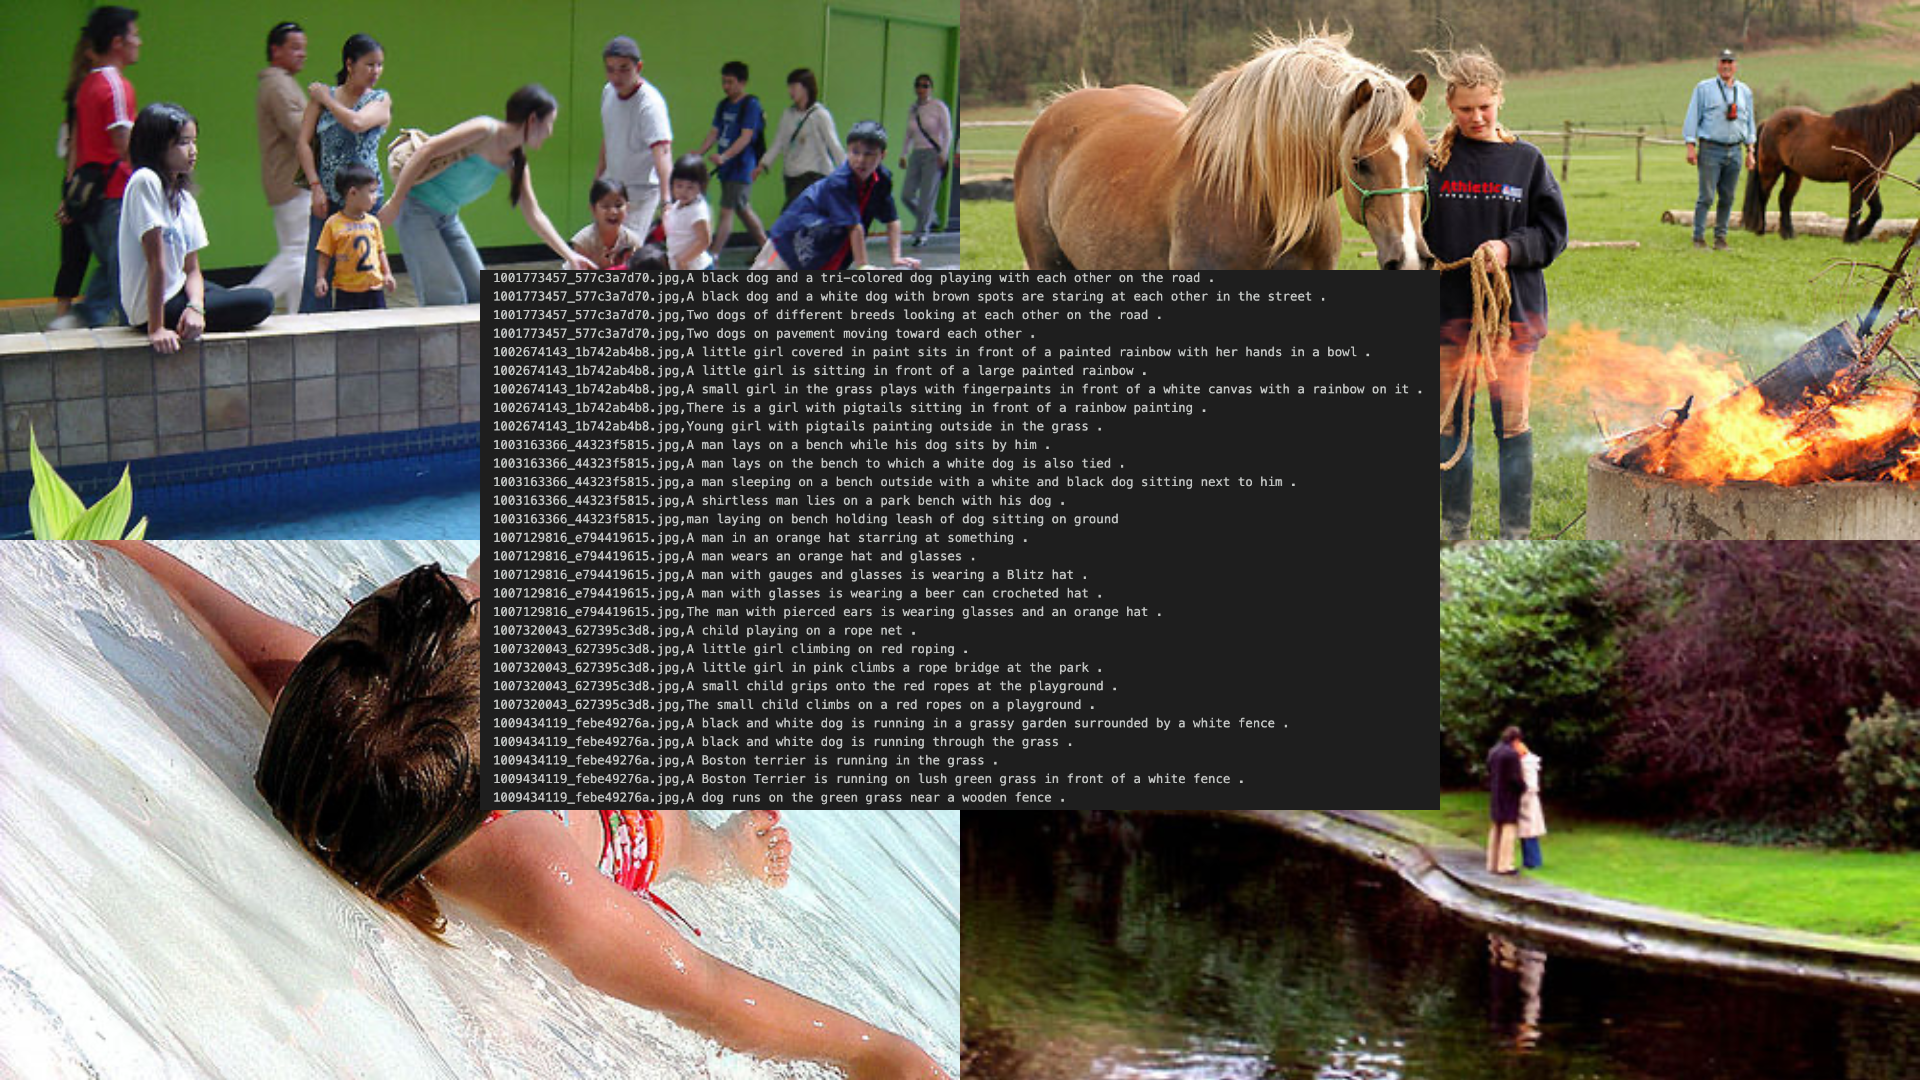
\includegraphics[width=.9\textwidth]{res/flickr8k.png}
    \caption{Example images and captions from the flickr8k dataset.}
    \label{fig:flickr8k}
\end{figure}

\subsection{Splitting the Data}\label{sec:splitting}
A predefined fixed split of the dataset into training, validation, and test sets is used. These datasets are stored in separate \textit{CSV} files.
\par The training set contains 80\% of the data, the validation set 10\%, and the test set 10\%. This split is fixed to ensure reproducibility and comparability of the results.


\subsection{Preprocessing}\label{sec:preprocessing}
The models require the images and the captions to be in a suitable format.

\subsubsection{Image Encoder}\label{sec:image-encoder}
Contrary to the usual approach, the encoding is applied as part of the preprocessing to save computational resources and simplify the model.
\par EfficientNet is used over other models due to its high performance compared to ResNet, for example. The model is pre-trained on the ImageNet dataset and used to extract features from the images. We use the B0 variant because it strikes a balance between computational efficiency and accuracy \cite{tan2019efficientnet}.

\subsubsection{Images}\label{sec:images}
The raw \textit{JPEG} images are loaded using the \textbf{PIL} library and preprocessed as follows:
\begin{enumerate}
    \item Resize the images to 224x224 pixels.
    \item Normalize the pixel values to the range [0, 1].
    \item Encode the images as tensors of the dimension (224, 224, 3).
    \item Use a pre-trained \texttt{EfficientNet B0} model to extract features from the images resulting in a tensor of the dimension (1280).
\end{enumerate}

\subsubsection{Vocabulary}\label{sec:vocabulary}
\begin{quote}\center Configurable: \texttt{SIZE}, \texttt{THRESHOLD} \end{quote}
To encode the captions, a vocabulary of words is created from the captions and each word is mapped to an index. Special tokens are added for padding, unknown tokens, start, and end of the sequence. The vocabulary size is limited to \texttt{SIZE} and words with a frequency below \texttt{THRESHOLD} are replaced by the unknown token.

\begin{table}[H]
    \begin{tabular}{c|cccccccc}
        \textbf{Word}  & $<$pad$>$ & $<$unknown$>$ & $<$start$>$ & $<$end$>$ & is & and & dog & with \\
        \textbf{Index} & 0         & 1             & 2           & 3         & 4  & 5   & 6   & 7
    \end{tabular}
    \caption{Example vocabulary with special tokens. \label{tab:vocabulary}}
\end{table}

\subsubsection{Captions}\label{sec:captions}
\begin{quote}\center Configurable: \texttt{CAPTION\_LEN}\end{quote}
The raw captions are loaded from the \textit{CSV} file and preprocessed as follows:
\begin{enumerate}
    \item Convert the captions to lowercase.
    \item Tokenize the captions.
    \item Encode the captions using our Vocabulary \ref{sec:vocabulary}.
    \item Pad or truncate the captions to a fixed length \texttt{CAPTION\_LEN}.
    \item Convert the captions to one-dimensional tensors with a specified \texttt{CAPTION\_LEN}.
\end{enumerate}

\subsection{Dataset and Dataloader}\label{sec:dataset}
To use the data efficiently within the model, a custom \textbf{PyTorch}-based Dataset with \textbf{PyTorch}'s DataLoader is used
\par The Dataset loads the images and captions and returns them as a tuple.
\par The DataLoader then batches the data.



\section{Models}\label{sec:models}
\begin{quote}\center Configurable: \texttt{HIDDEN\_DIM}, \texttt{EMBEDDING\_DIM}, \texttt{NUM\_LAYERS}, \texttt{DROPOUT}\end{quote}
In our paper, different decoder models are used for experiments, while the encoder (refer to \ref{sec:image-encoder}) stays the same. Two RNNs, GRU and LSTM, and a Transformer (decoder) for decoding the captions are compared.
\par We use the \textbf{PyTorch} library to implement the models.

\subsection{GRU}\label{sec:gru}
Gated recurrent units are a popular simplified alternative to LSTMs \cite{cho2014gru}. The GRU model architecture is shown in Figure \ref{fig:gru}.
\par The model predicts each token in sequence. The hidden state is updated at each time step and used to predict the next token. The model is trained using teacher forcing, where the true target token is used as input to predict the next token.
\begin{figure}[H]
    \centering
    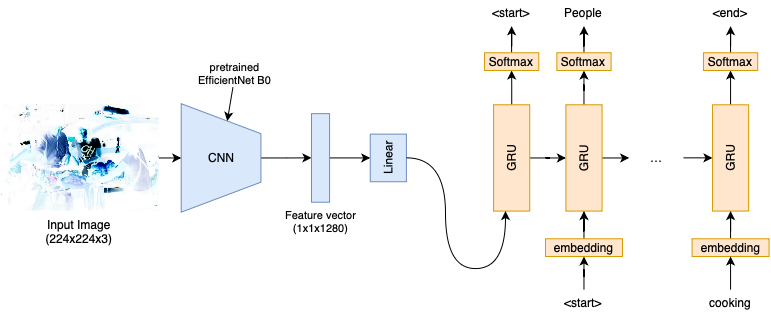
\includegraphics[width=.7\textwidth]{res/gru.png}
    \caption{The GRU model architecture.}\label{fig:gru}
\end{figure}

\subsection{LSTM}\label{sec:lstm}
Long Short-Term Memory networks are a type of RNN that can learn long-term dependencies \cite{hochreiter1997lstm}. The LSTM model architecture is shown in Figure \ref{fig:lstm}.
\par Like the GRU model, the LSTM model predicts each token in sequence. The hidden state is updated at each time step and used to predict the next token. The model is trained using teacher forcing.
\begin{figure}[H]
    \centering
    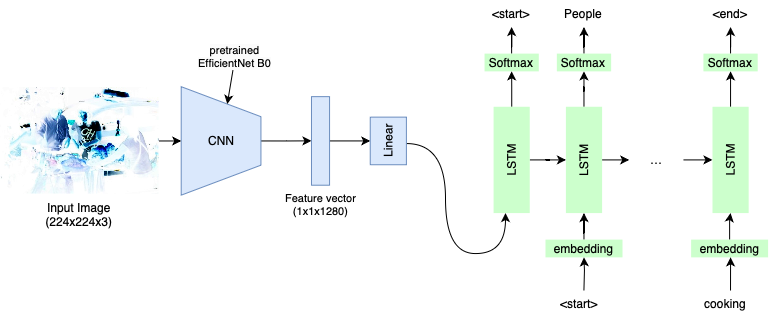
\includegraphics[width=.7\textwidth]{res/lstm.png}
    \caption{The LSTM model architecture.}\label{fig:lstm}
\end{figure}

\subsection{Transformer}\label{sec:transformer}
The Transformer model architecture is shown in Figure \ref{fig:transformer}. The model is based on the original paper \cite{vaswani2017attention}.
\par Contrary to the RNNs, the Transformer predicts the whole sequence at once. The model uses self-attention mechanisms to capture dependencies between words in the sequence. The model is trained using teacher forcing.
\begin{figure}[H]
    \centering
    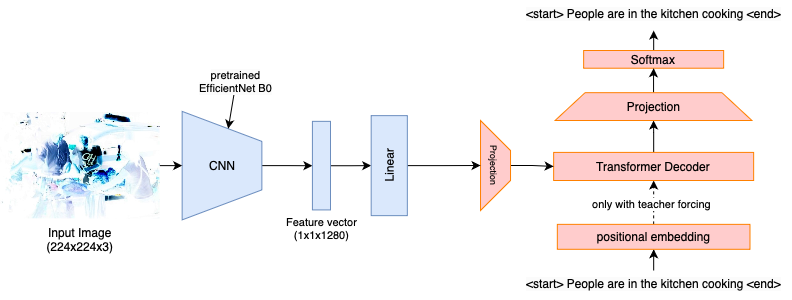
\includegraphics[width=.7\textwidth]{res/transformer.png}
    \caption{The Transformer model architecture.}\label{fig:transformer}
\end{figure}



\section{Experiments}\label{sec:experiments}
The research question we are trying to answer is: \textit{Which decoder model performs best for the task of image captioning?}

\subsection{Training}\label{sec:training}
\begin{quote}\center Configurable: \texttt{EPOCHS}, \texttt{PATIENCE}, \texttt{BATCH\_SIZE}, \texttt{LEARNING\_RATE}\end{quote}
\par The models are trained using the Adam optimizer and the CrossEntropyLoss function.
\par The models are trained for a number of epochs \texttt{EPOCHS}. If the \texttt{PATIENCE} hyperparameter is set and the validation loss does not improve for \texttt{PATIENCE} epochs, the training is stopped early. Batching makes training more efficient and can be adjusted with the \texttt{BATCH\_SIZE} hyperparameter.

\subsection{Evaluation metrics}\label{sec:evaluation-metrics}
To evaluate the models, BLEU, METEOR, and NIST scores are used. These are common metrics used in machine translation and image captioning tasks.
\begin{enumerate}
    \item BLEU (Bilingual Evaluation Understudy) is a metric that compares the generated captions to the reference captions. It measures the n-gram overlap between the generated and reference captions \cite{papineni2002bleu}. We use the BLEU-4 score, meaning up to 4-grams are considered.
    \item METEOR (Metric for Evaluation of Translation with Explicit ORdering) is a metric that considers the generated and reference captions as sequences of words. It uses a harmonic mean of precision and recall \cite{banerjee2005meteor}.
    \item NIST (Normalized Information Retrieval Metric) is a metric that rewards longer n-grams more than shorter ones. It is based on the BLEU metric \cite{doddington2002nist}. We use the NIST-4 score, meaning up to 4-grams are considered.
\end{enumerate}

\subsection{Results}\label{sec:results}
Our experiments use the hyperparameters shown in Table \ref{tab:hyperparameters}.
\begin{table}[H]
    \center
    \fontsize{8}{10}\selectfont
    \begin{tabular}{r|l}
        \texttt{CAPTION\_LEN}   & 20   \\
        \texttt{SIZE}           & 8000 \\
        \texttt{THRESHOLD}      & 2    \\
        \texttt{HIDDEN\_DIM}    & 512  \\
        \texttt{EMBEDDING\_DIM} & 256  \\
        \texttt{NUM\_LAYERS}    & 2    \\
        \texttt{DROPOUT}        & .1   \\
        \texttt{EPOCHS}         & 100  \\
        \texttt{PATIENCE}       & None \\
        \texttt{BATCH\_SIZE}    & 64   \\
        \texttt{LEARNING\_RATE} & 1e-3
    \end{tabular}
    \caption{Hyperparameters used in the experiments.}\label{tab:hyperparameters}
\end{table}

The training and validation loss for the different models are shown in Figure \ref{fig:loss}.
\begin{figure}[H]
    \centering
    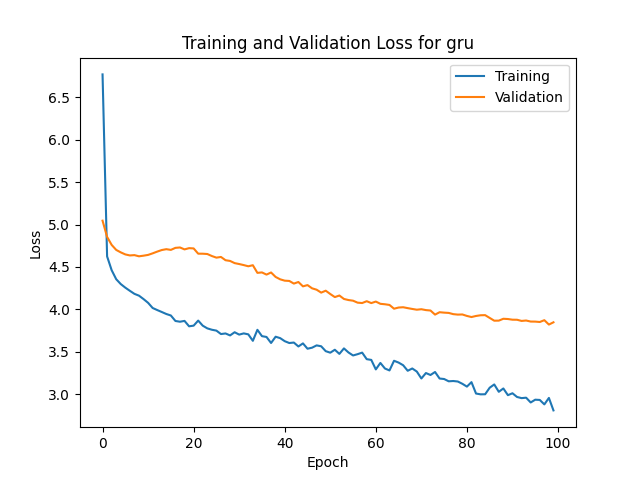
\includegraphics[width=.3\textwidth]{res/training-gru.png}
    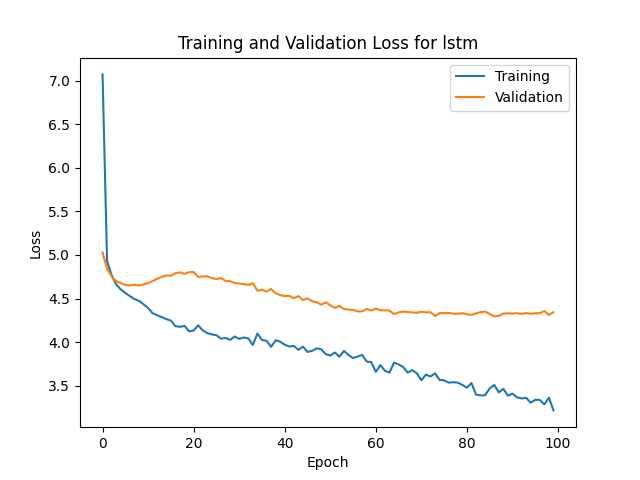
\includegraphics[width=.3\textwidth]{res/training-lstm.png}
    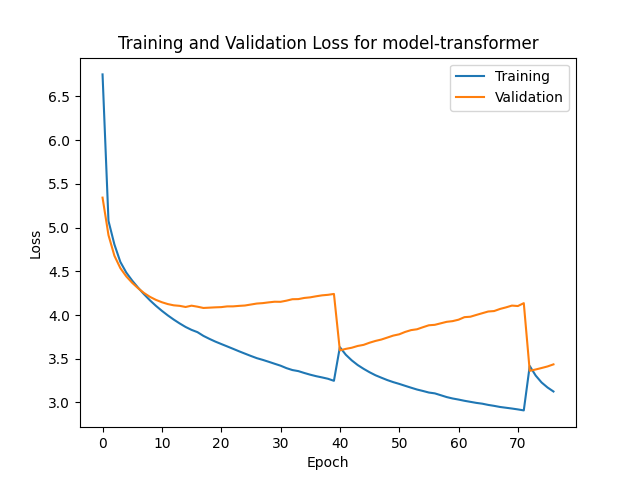
\includegraphics[width=.3\textwidth]{res/training-transformer.png}
    \caption{Training and validation loss for the different models.}\label{fig:loss}
\end{figure}
Training the models took approximately 20 hours per model on a single GPU. The validation loss is similar for all models. The weird shape of the Transformer losses is due to interrupted training.

The results of the evaluation metrics are shown in Table \ref{tab:results} and Figure \ref{fig:results}.
\begin{figure}[H]
    \centering
    \begin{minipage}{0.4\textwidth}
        \begin{table}[H]
            \centering
            \fontsize{8}{10}\selectfont
            \begin{tabular}{c|c|c|c}
                            & \textbf{BLEU-4} & \textbf{METEOR} & \textbf{NIST-4} \\
                GRU         & .0511           & .1551           & 1.0202          \\
                LSTM        & .0541           & .1537           & .9137           \\
                Transformer & .0183           & .0956           & .6013
            \end{tabular}
            \caption{Evaluation metrics.}\label{tab:results}
        \end{table}
    \end{minipage}
    \hfill
    \begin{minipage}{0.5\textwidth}
        \centering
        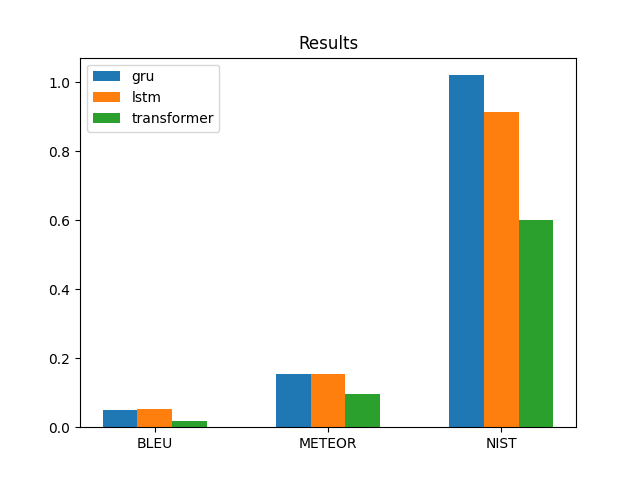
\includegraphics[width=.9\textwidth]{res/metrics.png}
        \caption{Evaluation metrics.}\label{fig:results}
    \end{minipage}
\end{figure}

The results show that the LSTM and GRU models perform roughly the same, while the Transformer model performs worse in all metrics. This is contrary to expectations, as Transformers have shown remarkable performance in various NLP tasks.
\par This is likely due to the limited training time and computational resources. Also, the Transformer predicts the whole sequence at once, which might be suboptimal for image captioning tasks.
\par Compared to other research, our results are much worse. \cite{vinyals2015show} achieved a BLEU score of  27.7, for example, and \cite{xu2015show} achieved a METEOR score of 24.3.
\par This might have several reasons: \begin{enumerate}
    \item \textbf{Smaller Dataset}: The flickr8k dataset is smaller than other datasets like MS COCO, which is used in \cite{vinyals2015show} and \cite{xu2015show}.
    \item \textbf{Encoder}: The EfficientNet B0 model is less powerful than other models like ResNet, for example \cite{he2016deep}.
    \item \textbf{No attention mechanisms}: The models used in this paper do not use attention mechanisms, which are crucial for image captioning \cite{xu2015show}
    \item \textbf{Limited training time}: The models were trained for a limited number of epochs due to computational constraints.
\end{enumerate}



\section{Conclusion}\label{sec:conclusion}

This paper presents our experiments with different decoder models for the task of image captioning. The flickr8k dataset is used and the models are evaluated using BLEU, METEOR, and NIST scores.
\par Our results show that the LSTM and GRU models outperform the Transformer model in all metrics given the limited training time and computational resources.
\par In the future, further experiments should be conducted with
\begin{enumerate}
    \item other encoder models, like ResNet or VGG.
    \item varying the batch size or learning rate to optimize the training process.
    \item different datasets, like flickr30k and MS COCO.
\end{enumerate}
These can build on the code provided in this paper and extend the research on image captioning.



%%%%%%%%%%%%%%%%%%%%%%%%%%%%%%%%%%%%%%
% References
%%%%%%%%%%%%%%%%%%%%%%%%%%%%%%%%%%%%%%
\newpage
\thispagestyle{empty}

\fontsize{12}{14}\selectfont
\bibliographystyle{acm}
\bibliography{bib}

\end{document}